\chapter{Lecture 20: Harmonic Functions}

\begin{definition}
    [Harmonic Functions]
    if $D \subseteq \mathbb{C} = \mathbb{R}^2$ is open, then $u: D \rightarrow \mathbb{R}$ is \textbf{harmonic} if it satisfies \underline{Laplace's equation}:
    $$\Delta u = \frac{\partial^2 u}{\partial x^2} + \frac{\partial^2 u}{\partial y^2} = 0$$
\end{definition}

\begin{remark}
    Harmonic functions are ubiquitous in physical applications.\\
    for example, a harmonic function $u$ may describe:
    \begin{itemize}
        \item The steady state temperature distribution $\mathbb{R}^2$.
              \begin{itemize}
                  \item Temperature at $x$ is $\phi(x), \quad x \in \partial D = \gamma$
              \end{itemize}
    \end{itemize}

    \begin{itemize}
        \item Electrostatic potential energy
        \item Planar stress
        \item Potential energy in an ideal fluid
        \item In general, harmonic functions can represent potential energy
        \item Particle motion where we look to minimize potential energy as fast as possible
              \begin{itemize}
                  \item $x(t)$ ais a trajectory of a particle in $\mathbb{R}^2$
                  \item $\dot{x}(t) = -\nabla u(x(t))$ where $u$ is a harmonic function
              \end{itemize}
    \end{itemize}
\end{remark}

\begin{proposition}
    [Harmonic Functions Representing Particle motion]
    Say $x(t)$ is a trajectory of a particle in $\mathbb{R}^2$ and $\dot{x}(t) = -\nabla u(x(t))$ where $u$ is a harmonic function.\\
    We can try to find a function $v$ such that:
    \begin{align*}
        \nabla v & = (\nabla u)^\perp = \begin{pmatrix}
                                            -\frac{\partial u}{\partial y} \\
                                            \frac{\partial u}{\partial x}
                                        \end{pmatrix} \\
    \end{align*}
    Therefore $v$ must satisfy:
    \begin{align*}
        \frac{\partial v}{\partial x} & = -\frac{\partial u}{\partial y} \\
        \frac{\partial v}{\partial y} & = \frac{\partial u}{\partial x}
    \end{align*}
    Which are the Cauchy-Riemann equations!\\
    $v$ is called the \textbf{conjugate harmonic function} of $u$. The level sets of $\{v = \text{const}\}$ are trajectories of the particle $u$.\\

    If $D = \{|z - z_0| < r\}$ is a disk, then
    \begin{align*}
        v(x, y) & = - \int_{x_0}^x \frac{\partial u}{\partial y}(t,y_0) dt + \int_{y_0}^y \frac{\partial u}{\partial x}(x_0, t) dt \\
    \end{align*}
    Then $f = u + iv$ is \underline{analytic} in $D$.
\end{proposition}

\begin{theorem}
    A real-valued function is harmonic if and only if, on every disk, it is the real part of the analytic function.\\
    Therefore, if I have a harmonic function, I can find an analytic function whose real part is the harmonic function and whose imaginary part is the conjugate harmonic function. Conversely, if I have an analytic function, I can find a harmonic function whose real part is the real part of the analytic function.
\end{theorem}

\begin{example}
    $u(x, y) = \frac{1}2 \log(x^2 + y^2)$ is harmonic in $\{0 < x^2 + y^2 < 1\}$. Is it the real part of an analytic function?\\

    No, it is not the real part of an analytic function defined on $\{ 0 < |z| < 1\}$, because $u = \Re(\log z)$, but $\log z = \log |z| + i\arg z$ is not continuous on $\{0 < |z| < 1\}$ because $\arg z$ is not continuous on $\{0 < |z| < 1\}$. This is due to the branch cut of the logarithm function, and it's an exception to the theorem.

\end{example}

\begin{remark}
    Due to the earlier theorem, properties of analytic functions are very closely (often equivalent) to properties of harmonic functions.
\end{remark}

\begin{lemma}
    [Maximum Modulus Principle for Harmonic Functions]
    if $u: D \rightarrow \mathbb{R}$ is harmonic and $D$ is open and connected, then $u$ cannot have a local max/min in $D$, unless $u$ is constant.
    $$ \forall x \in D, \quad u(x) < \max_{\partial D} u \quad \text{ if }u \text{ not constant}$$
    $$ \forall x \in D, \quad u(x) = \max_{\partial D} u \text{ iff } u \text{ is constant on } D$$
\end{lemma}
\begin{proof}
    I'm not going to pretend I understand this proof, but here it is:\\
    Suppose $x_* \in D$ is a local max of $u$. Then $\text{Hess } u(x_*)$ is negative semi-definite, so:
    \begin{align*}
        0 = \Delta u(x_*) = \text{Tr }( \text{Hess } u(x_*)) \leq 0
    \end{align*}

\end{proof}

\begin{lemma}
    [Mean Value Property]
    if $u$ is harmonic on $\{ |z - z_0| < 2r\}$, then
    \begin{align*}
        u(z_0) & = \frac{1}{2\pi} \int_0^{2\pi} u(z_0 + re^{i\theta}) d\theta                           \\
               & = \text{The average of } u \text{ on the circle of radius } r \text{ centered at } z_0
    \end{align*}
    \textbf{In fact:} The mean value property is \underline{equivalent} to being harmonic.
\end{lemma}

\begin{lemma}
    If $u: D \to \mathbb{R}$ is harmonic on domain $D$ and $\phi (\xi) : \tilde{D} \rightarrow D$ is analytic then $u \circ \phi$ is harmonic on $\tilde{D}$.
\end{lemma}

\section{Harmonic Functions as Energy Minimizer}
\begin{figure}[H]
    \centering
    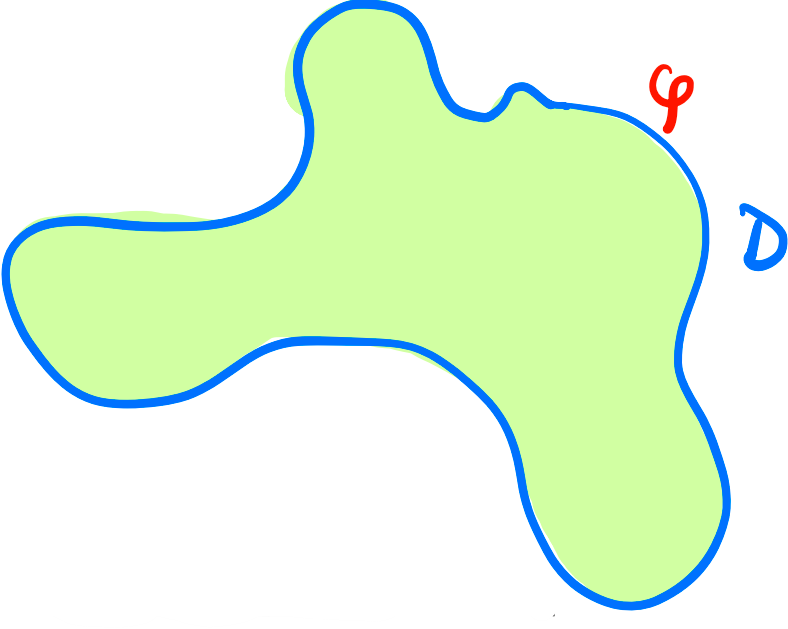
\includegraphics[scale=0.5]{LECTURE_20/domain.png}
    \caption{Heat distribution on a wire}
\end{figure}
\begin{proposition}
    Let $D \subset \mathbb{R}^2$ be a domain, $\gamma = \partial D$, and $\phi : D \rightarrow \mathbb{R}$ be continuous.

    You can think of $\partial D$ as a wire with a specified temperature, and $\phi$ is the heat distribution along $D$\\
    The natural energy (Dirichlet energy) associated with a function $u: D \rightarrow \mathbb{R} \quad | \quad u|_{\partial D} = \phi$ is:
    \begin{align*}
        \xi(u)                   & = \int_D |\nabla u|^2 dxdy                                                                                                   \\
                                 & = \int_D \left[ \left( \frac{\partial u}{\partial x} \right)^2 + \left( \frac{\partial u}{\partial y} \right)^2 \right] dxdy \\\\
        \therefore \text{ if } u & \sim Kg (\frac{m^2}{s^2}) \quad \text{has units of energy}                                                                   \\
        \nabla u                 & \sim (\frac{Kgm}{s^2}) \quad \text{force}                                                                                    \\
        |\nabla u|^2             & \sim (\frac{Kg^2m^2}{s^4}) \quad \text{energy density}                                                                       \\
        \sqrt{\xi}               & \sim (\frac{Kg m}{s^2}) \quad \text{energy}                                                                                  \\
    \end{align*}
    \begin{itemize}
        \item $u(x, y)$ is our temperature distribution
        \item $\xi(u)$ Represents the total energy of $u$ in $D$, it measure the smoothness of $u$. Essentially, the magnitude of the gradient of $u$ at every point in $D$.
        \item We want to find $u$ such that $u|_{\partial D} = \phi$ and $\xi(u)$ is minimized (because heat spreads out, thus we should reduce the magnitude of the gradient).
        \item This is a boundary value problem.
    \end{itemize}
    The physical temperature distribution should \underline{minimize} $\xi(u)$ over all functions on $D$ such that $u|_{\partial D} = \phi$. We say $u$ is minimized if, for any $\psi : D \rightarrow \mathbb{R}$ such that $\psi|_{\partial D} = 0$, we have:
    \begin{align*}
        \xi(u + t\psi)                                                                                                  & \geq \xi(u) \quad \forall t \in \mathbb{R} \\
        \int_D |\nabla u|^2 \; dxdy + 2t \int_D \nabla u \cdot \nabla \psi \; dxdy + t^2 \int_D |\nabla \psi|^2 \; dxdy & =                                          \\
        \xi (u) + 2t\int_D \nabla u \cdot \nabla \psi \; dxdy + t^2 \int_D |\nabla \psi|^2 \; dxdy                      & \geq \xi(u)
    \end{align*}
    We can determine that $\int_D \nabla u \cdot \nabla \psi \; dxdy = 0$ By considering that if $\xi(u)$ is minimized, then $\frac{d}{dt} \xi(u + t\psi) = 0$ at $t = 0$ because a minimum is a critical point.
    \begin{align}
        \frac{d}{dt} \xi(u + t\psi) & = \frac{d}{dt}\left[ \int_D |\nabla u|^2 \; dxdy + 2t \int_D \nabla u \cdot \nabla \psi \; dxdy + t^2 \int_D |\nabla \psi|^2 \; dxdy \right]_{t = 0} \\
        0                           & = 2\int_D \nabla u \cdot \nabla \psi \; dxdy
    \end{align}
    Let's integrate $\int_D \nabla u \cdot \nabla \psi \; dxdy$ by parts:
    \begin{align*}
        0 & = \int_D \nabla u \cdot \nabla \psi \;dxdy                                                          \\
          & = \int_D\nabla \cdot (\psi \nabla u)   \; dxdy                                                      \\
          & = \int_{\partial D} \psi \nabla u \cdot \vec{\eta} dS - \int_D \psi \nabla \cdot (\nabla u) \; dxdy
    \end{align*}
    Where $\vec{\eta}$ is the outward normal to $\partial D$, but since $\psi|_{\partial D} = 0$, the first term is 0, and so:
    \begin{align*}
        0 & = \int_D \psi \nabla \cdot (\nabla u) \; dxdy \\
          & = \int_D \psi \Delta u \; dxdy
    \end{align*}
    But this should hold for \textbf{all} $\psi$ where $\psi|_{\partial D} = 0$, so $\Delta u = 0$.
    \begin{figure}[H]
        \centering
        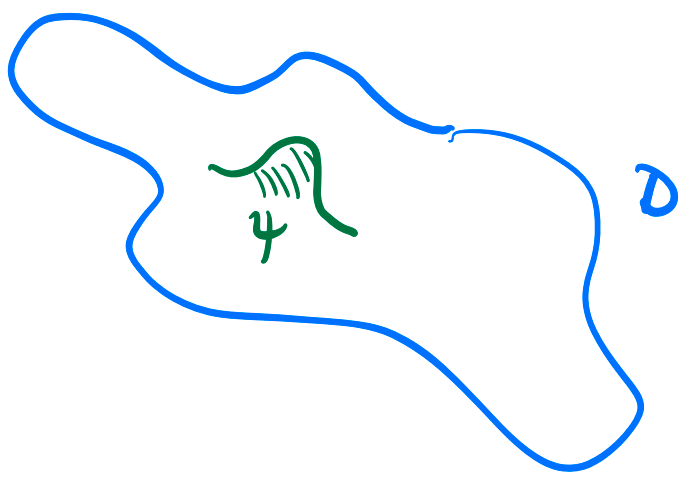
\includegraphics[scale=0.5]{LECTURE_20/boundary.png}
        \caption{Boundary of domain $D$}
    \end{figure}

    For most physical problems, we expect the energy should satisfy:
    \begin{align*}
        V(x) \sim |x|^2 \quad \text{near a minimizer}
    \end{align*}
    Where $V$ is the potential energy (or energy density) of the system.
    \begin{align*}
        \int_D V(\nabla u) dx = \int_D |\nabla u|^2 dx
    \end{align*}
    Which is why harmonic functions appear so often in physics and engineering.
\end{proposition}